\documentclass[12pt]{article}
\usepackage[T1]{fontenc}
\usepackage[T1]{polski}
\usepackage[cp1250]{inputenc}
\newcommand{\BibTeX}{{\sc Bib}\TeX} 
\usepackage{graphicx}
\usepackage{amsfonts}
\usepackage{float}

\setlength{\textheight}{21cm}

\title{{\bf Zadanie nr 2 - Pr�bkowanie i kwantyzacja}\linebreak
Cyfrowe Przetwarzanie Sygnal�w}
\author{Justyna Hubert, 210200 \and Karol Podlewski, 210294}
\date{17.04.2019}

\begin{document}
\clearpage\maketitle
\thispagestyle{empty}
\newpage
\setcounter{page}{1}


%%%%%%%%%%%%%%%%%%%%%%%%%%%%%%%%%%%%%%%%%%%%%%%%%%%%%%%%%%%%
%% CEL ZADANIA
%%%%%%%%%%%%%%%%%%%%%%%%%%%%%%%%%%%%%%%%%%%%%%%%%%%%%%%%%%%%
\section{Cel zadania}
Celem �wiczenia jest zapoznanie sie z praktycznymi aspektami filtracji, korelacji oraz operacji splotu.
%%%%%%%%%%%%%%%%%%%%%%%%%%%%%%%%%%%%%%%%%%%%%%%%%%%%%%%%%%%%
%% WSTEP TEORETYCZNY
%%%%%%%%%%%%%%%%%%%%%%%%%%%%%%%%%%%%%%%%%%%%%%%%%%%%%%%%%%%%
\section{Wstep teoretyczny}
Jest to usprawniony program z zadania 1 oraz 2, dostosowany do instrukcji z zadania trzeciego ~\cite{instrukcja}. \\

Zadanie polegalo na zaimplementowaniu algorytmu, kt�ry umo�liwi projektowanie filtr�w dolnoprzepustowycho zadanej liczbie wsp�lczynnik�wi zadanej czestotliwosci obciecia z wykorzystaniem okna prostokatnego, zastosowaniu dodatkowych okien:
\begin{itemize}
	\item (O1) okno Hamminga,
	\item (O2) okno Hanninga,
	\item (O3) okno Blackmana,
\end{itemize}

Ponadto, w ramach realizacji �wiczenia nale�alo zaprojektowac filtr z mo�liwoscia wyboru funkcji okna i parametr�w filtru jak wy�ej:
\begin{itemize}
	\item (F1) srodkowoprzepustowy,
	\item (F2) g�rnoprzepustowy,
\end{itemize} 

Nale�alo tak�e zaimplementowac operacje filtracji podstawiajac odpowiedz impulsowa filtru do wzoru na splot, zademonstrowac efekt filtracji na arbitralnie wybranych sygnalach testowych. Ponadto, wymagana jest implementacja operacji korelacji dla dowolnych dw�ch sygnal�w dyskretnych o arbitralnie podanych ilosciach pr�bek wzbogacone o dwa obligatoryjne warianty:
\begin{itemize}
	\item implementacje bezposrednia,
	\item implementacje z u�yciem splotu,
\end{itemize}

Celem czesci zadania zwiazanej z zastosowaniem analizy korelacyjnej (pomiaru dlugosci) byla symulacja dzialania korelacyjnego czujnika odleglosci. 


\pagebreak

%%%%%%%%%%%%%%%%%%%%%%%%%%%%%%%%%%%%%%%%%%%%%%%%%%%%%%%%%%%%
%% SEKCJA EKSPERYMENT�W
%%%%%%%%%%%%%%%%%%%%%%%%%%%%%%%%%%%%%%%%%%%%%%%%%%%%%%%%%%%%
\section{Eksperymenty i wyniki}
Eksperymenty postanowilismy przeprowadzic na trzech rodzajach sygnal�w: sinusoidalnym, sinusoidalnym wyprostowanym jednopol�wkowo oraz tr�jkatnym. Zaprezentujemy proces konwersji analogowo-cyfrowej i cyfrowo-analogowej.

%%%%%%%%%%%%%%%%%%%%%%%%%%%%%%%%%%%%%%%%%%%%%%%%%%%%%%%%%%%%
%%%%%%%%%%%% EKSPERYMENT #1  
\subsection{Sygnal sinusoidalny}

\begin{figure}[H]
	\centering
		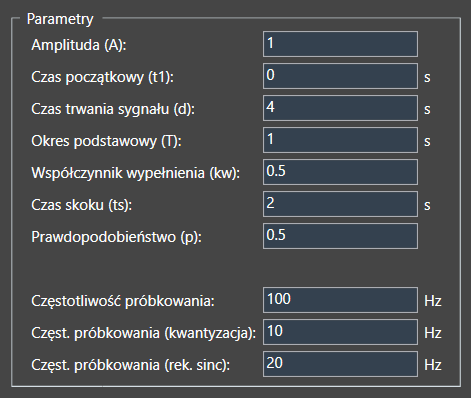
\includegraphics[width=0.7\textwidth]{{Rysunki/SinParametry.png}}
	\caption{Parametry, kt�re przyjmuje funkcja sinusoidalna.}
\end{figure}

\pagebreak

%%%%%%%%%%%%%%%%%%%%%%%%%%%%%%%%%%%%%%%%%%%%%%%%%%%%%%%%%%%%
%%%%%%%%%%%% EKSPERYMENT #2  
\subsection{Sygnal sinusoidalny}

\pagebreak

%%%%%%%%%%%%%%%%%%%%%%%%%%%%%%%%%%%%%%%%%%%%%%%%%%%%%%%%%%%%
%% WNIOSKI
%%%%%%%%%%%%%%%%%%%%%%%%%%%%%%%%%%%%%%%%%%%%%%%%%%%%%%%%%%%%
\section{Wnioski}
Aplikacja zostala napisana zgodnie z instrukcj� do zadania ~\cite{instrukcja}. Program poprawnie implementuje operacje splotu, filtracji oraz korelacji. Aplikacja zostala napisana w spos�b, aby umo�liwiaj�cy nam rozszerzenie jej o kolejne funkcjonalnosci

%%%%%%%%%%%%%%%%%%%%%%%%%%%%%%%%%%%%%%%%%%%%%%%%%%%%%%%%%%%%
%% BIBLIOGRAFIA
%%%%%%%%%%%%%%%%%%%%%%%%%%%%%%%%%%%%%%%%%%%%%%%%%%%%%%%%%%%%
\renewcommand\refname{Bibliografia}
\bibliographystyle{plain}
\bibliography{Zad2_Bibliografia}

\end{document}
